% -----------------------------------------------------------------------------
% Introdução
% -----------------------------------------------------------------------------


\chapter{Introdução}
\label{chap:introducao}

Edite e coloque aqui o seu texto introdutório do artigo.

A introdução deverá apresentar uma visão de conjunto do trabalho a ser realizado, com o apoio da literatura, situando-o no contexto do estado da arte da área científica específica, sua relevância no contexto da área inserida e sua importância específica para o avanço do conhecimento.

Deve ser dado destaque às contribuições efetivas do trabalho e sua relevância para a área de pesquisa.

É uma boa prática iniciar cada novo capítulo com uma breve texto introdutório (tipicamente, dois ou três parágrafos) que deve deixar claro o quê será discutido no capítulo, bem como a organização do capítulo. Também servirá ao propósito de "amarrar"{} ou "alinhavar"{}  o conteúdo deste capítulo com o conteúdo do capítulo imediatamente anterior - neste caso, contando  com o texto da seção de "Considerações finais"{}  do capítulo anterior.


\section{Leia esta seção antes de começar}
\label{sec:antesleiame}

Este documento é um \emph{template} \LaTeX{} que foi concebido, primariamente, para ser utilizado na redação de teses de doutorado, dissertações de mestrado, projetos de qualificação tanto de mestrado quanto de doutorado, escritos em português brasileiro (eventualmente, com partes em inglês) e em conformidade com as normas da ABNT.

Não obstante, ele também poderá ser utilizado, com ligeiras adaptações para a redação de outros trabalhos acadêmicos monográficos - \emph{e.g.}, trabalhos de conclusão de curso de graduação ou de especialização \emph{lato sensu}.

Para a produção deste \emph{template} foi necessário adaptar o arquivo {\ttfamily abntex2.cls}. Assim, foi produzido o arquivo {\ttfamily abntex2-cefetmg.cls} que define o \verb|documentclass| específico para o CEFET-MG.

Antes de começar a escrever o seu trabalho acadêmico utilizando este \emph{template}, é bom saber que há dois arquivos que você precisará editar para que a capa e a folha de rosto de seu trabalho sejam geradas. São eles os arquivos {\ttfamily capa.tex} e {\ttfamily folhaRosto.tex}, ambos no diretório  {\ttfamily ./01-elementos-pre-textuais}. No arquivo {\ttfamily capa.tex} você deverá informar o seu nome, título do trabalho acadêmico, se o documento será uma tese de doutorado ou dissertação de mestrado ou projeto de qualificação, nome de seu(s) orientador(es), e outras informações necessárias. Já o arquivo {\ttfamily folhaRosto.tex} contém apenas o texto padrão - definido pelo Programa de Pós-graduação - estabelecendo que este documento é um requisito parcial para a obtenção do título pretendido. Neste arquivo, você deverá apenas comentar as linhas que não se aplicam ao seu tipo de trabalho acadêmico. Ambos os arquivos são auto-explicativos.

A conversão automática de acentos proporcionada pela codificação UTF8 no \LaTeX{} funciona bem, para o corpo do texto. E apenas para isso. A razão é que aquilo que é digitado no corpo do texto usualmente não sofre conversão para maiúsculas/minúsculas ou vice-versa.

Todavia, há vários elementos do documento que sofrem conversão minúsculas/maiúsculas - por exemplo o conteúdo dos arquivos {\ttfamily .bib}, {\ttfamily capa.tex} e {\ttfamily folhaRosto.tex}, além de títulos de capítulos, seções, etc.. Para estes elementos, pelo menos, não acentue diretamente as palavras, use os comandos relacionados na \autoref{fig:acentos-latex}.

\begin{figure}[!htb]
    \centering
    \caption{Comandos para acentuação no \LaTeX}
    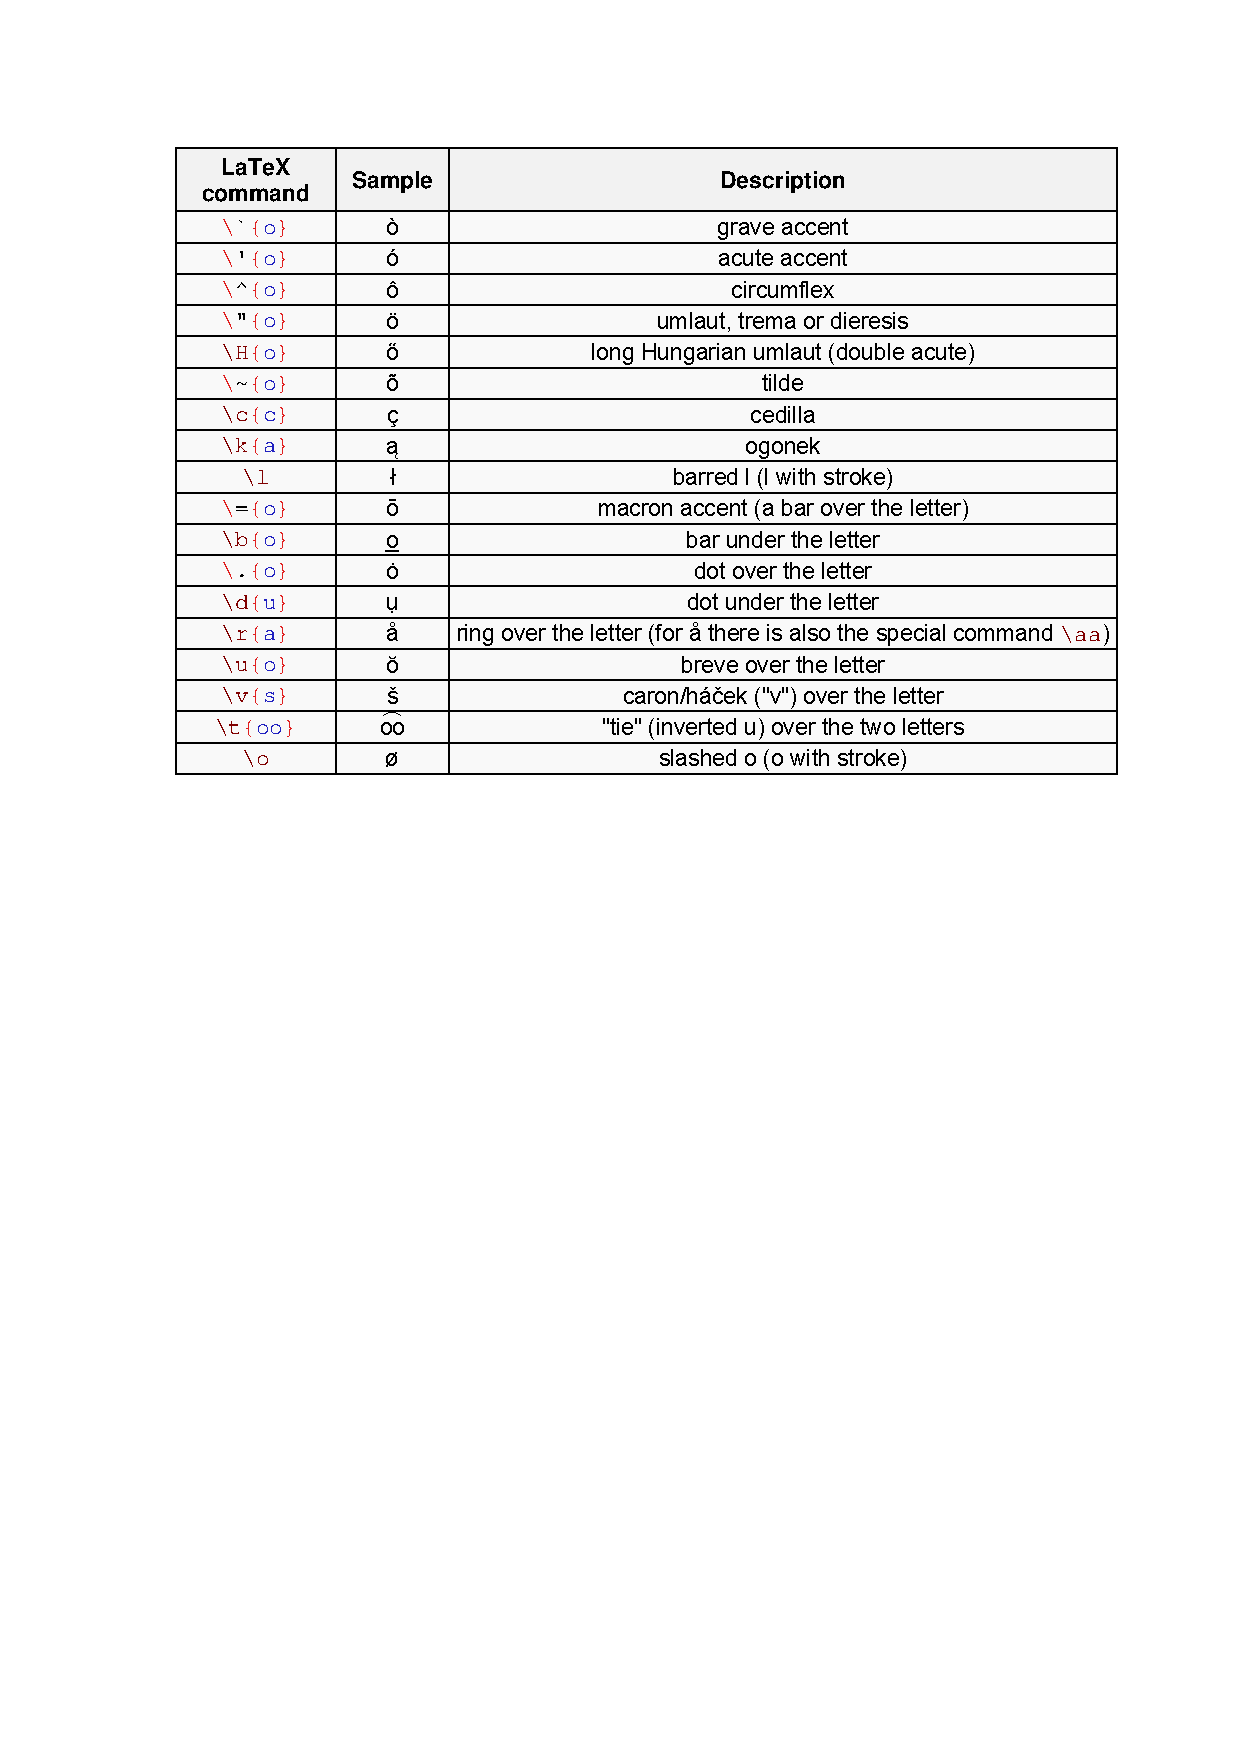
\includegraphics[width=0.8\textwidth]{./04-figuras/acentos-latex}
    \fonte{\href{http://en.wikibooks.org/wiki/LaTeX/Special_Characters}{http://en.wikibooks.org/wiki/LaTeX/Special\underline{ }Characters}}
    \label{fig:acentos-latex}
\end{figure}


Para a compilação de arquivos \TeX{} ou \LaTeX{} veja os comandos apresentados na \autoref{fig:comanCompilaTex}.


\begin{figure}[!htb]
    \centering
    \caption{Comandos para compilação de arquivos \TeX{} ou \LaTeX}
    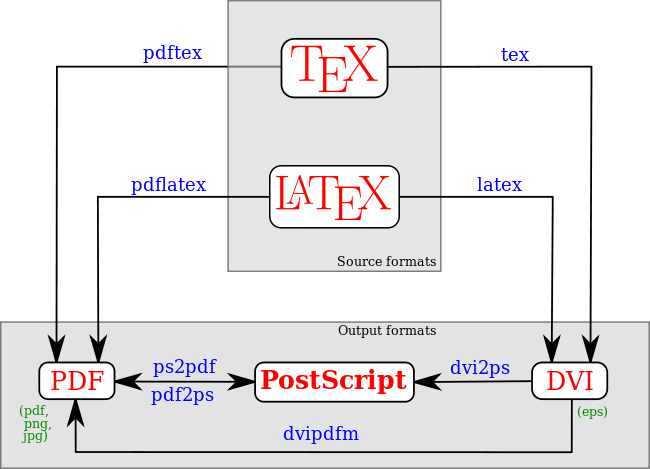
\includegraphics[width=0.8\textwidth]{./04-figuras/compilacao-tex}
    \fonte{\href{http://en.wikibooks.org/wiki/LaTeX/Basics}{http://en.wikibooks.org/wiki/LaTeX/Basics}}
    \label{fig:comanCompilaTex}
\end{figure}


A compilação para gerar um arquivo no formato pdf, incluindo corretamente as referências bibliográficas, deve ser realizada em quatro passos:

\begin{compactitem}
    \item \textbf{pdflatex} \verb|meuTrabalhoAcademico.tex|    -> gera um pdf, porém sem as referências, apenas indicando-as
    \item \textbf{bibtex} \verb|meuTrabalhoAcademico.tex|   -> varre o arquivo myrefs.bib e busca pelas referências utilizadas
    \item \textbf{pdflatex} \verb|meuTrabalhoAcademico.tex| -> insere as referências e chamadas nos locais apropriados
    \item \textbf{pdflatex} \verb|meuTrabalhoAcademico.tex| -> faz a compilação final, verificando tudo
\end{compactitem}

Alternativamente, poderá ser utilizado o comando \verb|makefile|, disponível na mesma pasta onde está o arquivo principal \verb|meuTrabalhoAcademico.tex|, que faz exatamente o mesmo que os quatro comandos supramencionados. No entanto atente para o fato de que , se você alterar o nome do arquivo \verb|meuTrabalhoAcademico.tex|, deverá também editar o arquivo \verb|makefile| para alterá-lo do mesmo modo.

Por fim, caso observe algum "\textit{bug}"{} ou qualquer outro tipo de falha ou mal comportamento neste modelo, comunique-nos para que possamos tentar corrigi-los em futuras atualizações deste modelo. Será melhor ainda se ao apontar uma falha ela venha acompanhada de uma proposta de solução.



\section{Justificativa}
\label{sec:justificativa}

Blá blá blá ....



\section{Motivação}
\label{sec:motivacao}

Blá blá blá ....



\section{Organização do trabalho}
\label{sec:organizacaoTrabalho}


Normalmente ao final da introdução é apresentada, em um ou dois parágrafos curtos, a organização do restante do trabalho acadêmico. Deve-se dizer o quê será apresentado em cada um dos demais capítulos.
